En esta secci\'on se muestra el avance obtenido al construir el circuito para el control del sistema de riego.
\section{Etapa 1: Sistema de Riego}
\subsection{Circuito del sistema de riego con raspberry}
En esta primera etapa se construy\'o un circuito en el que se implementaron los sensores para el monitero del sistema de riego como se puede observar en la figura \ref{r2}

\begin{figure}[H]
	\begin{center}
		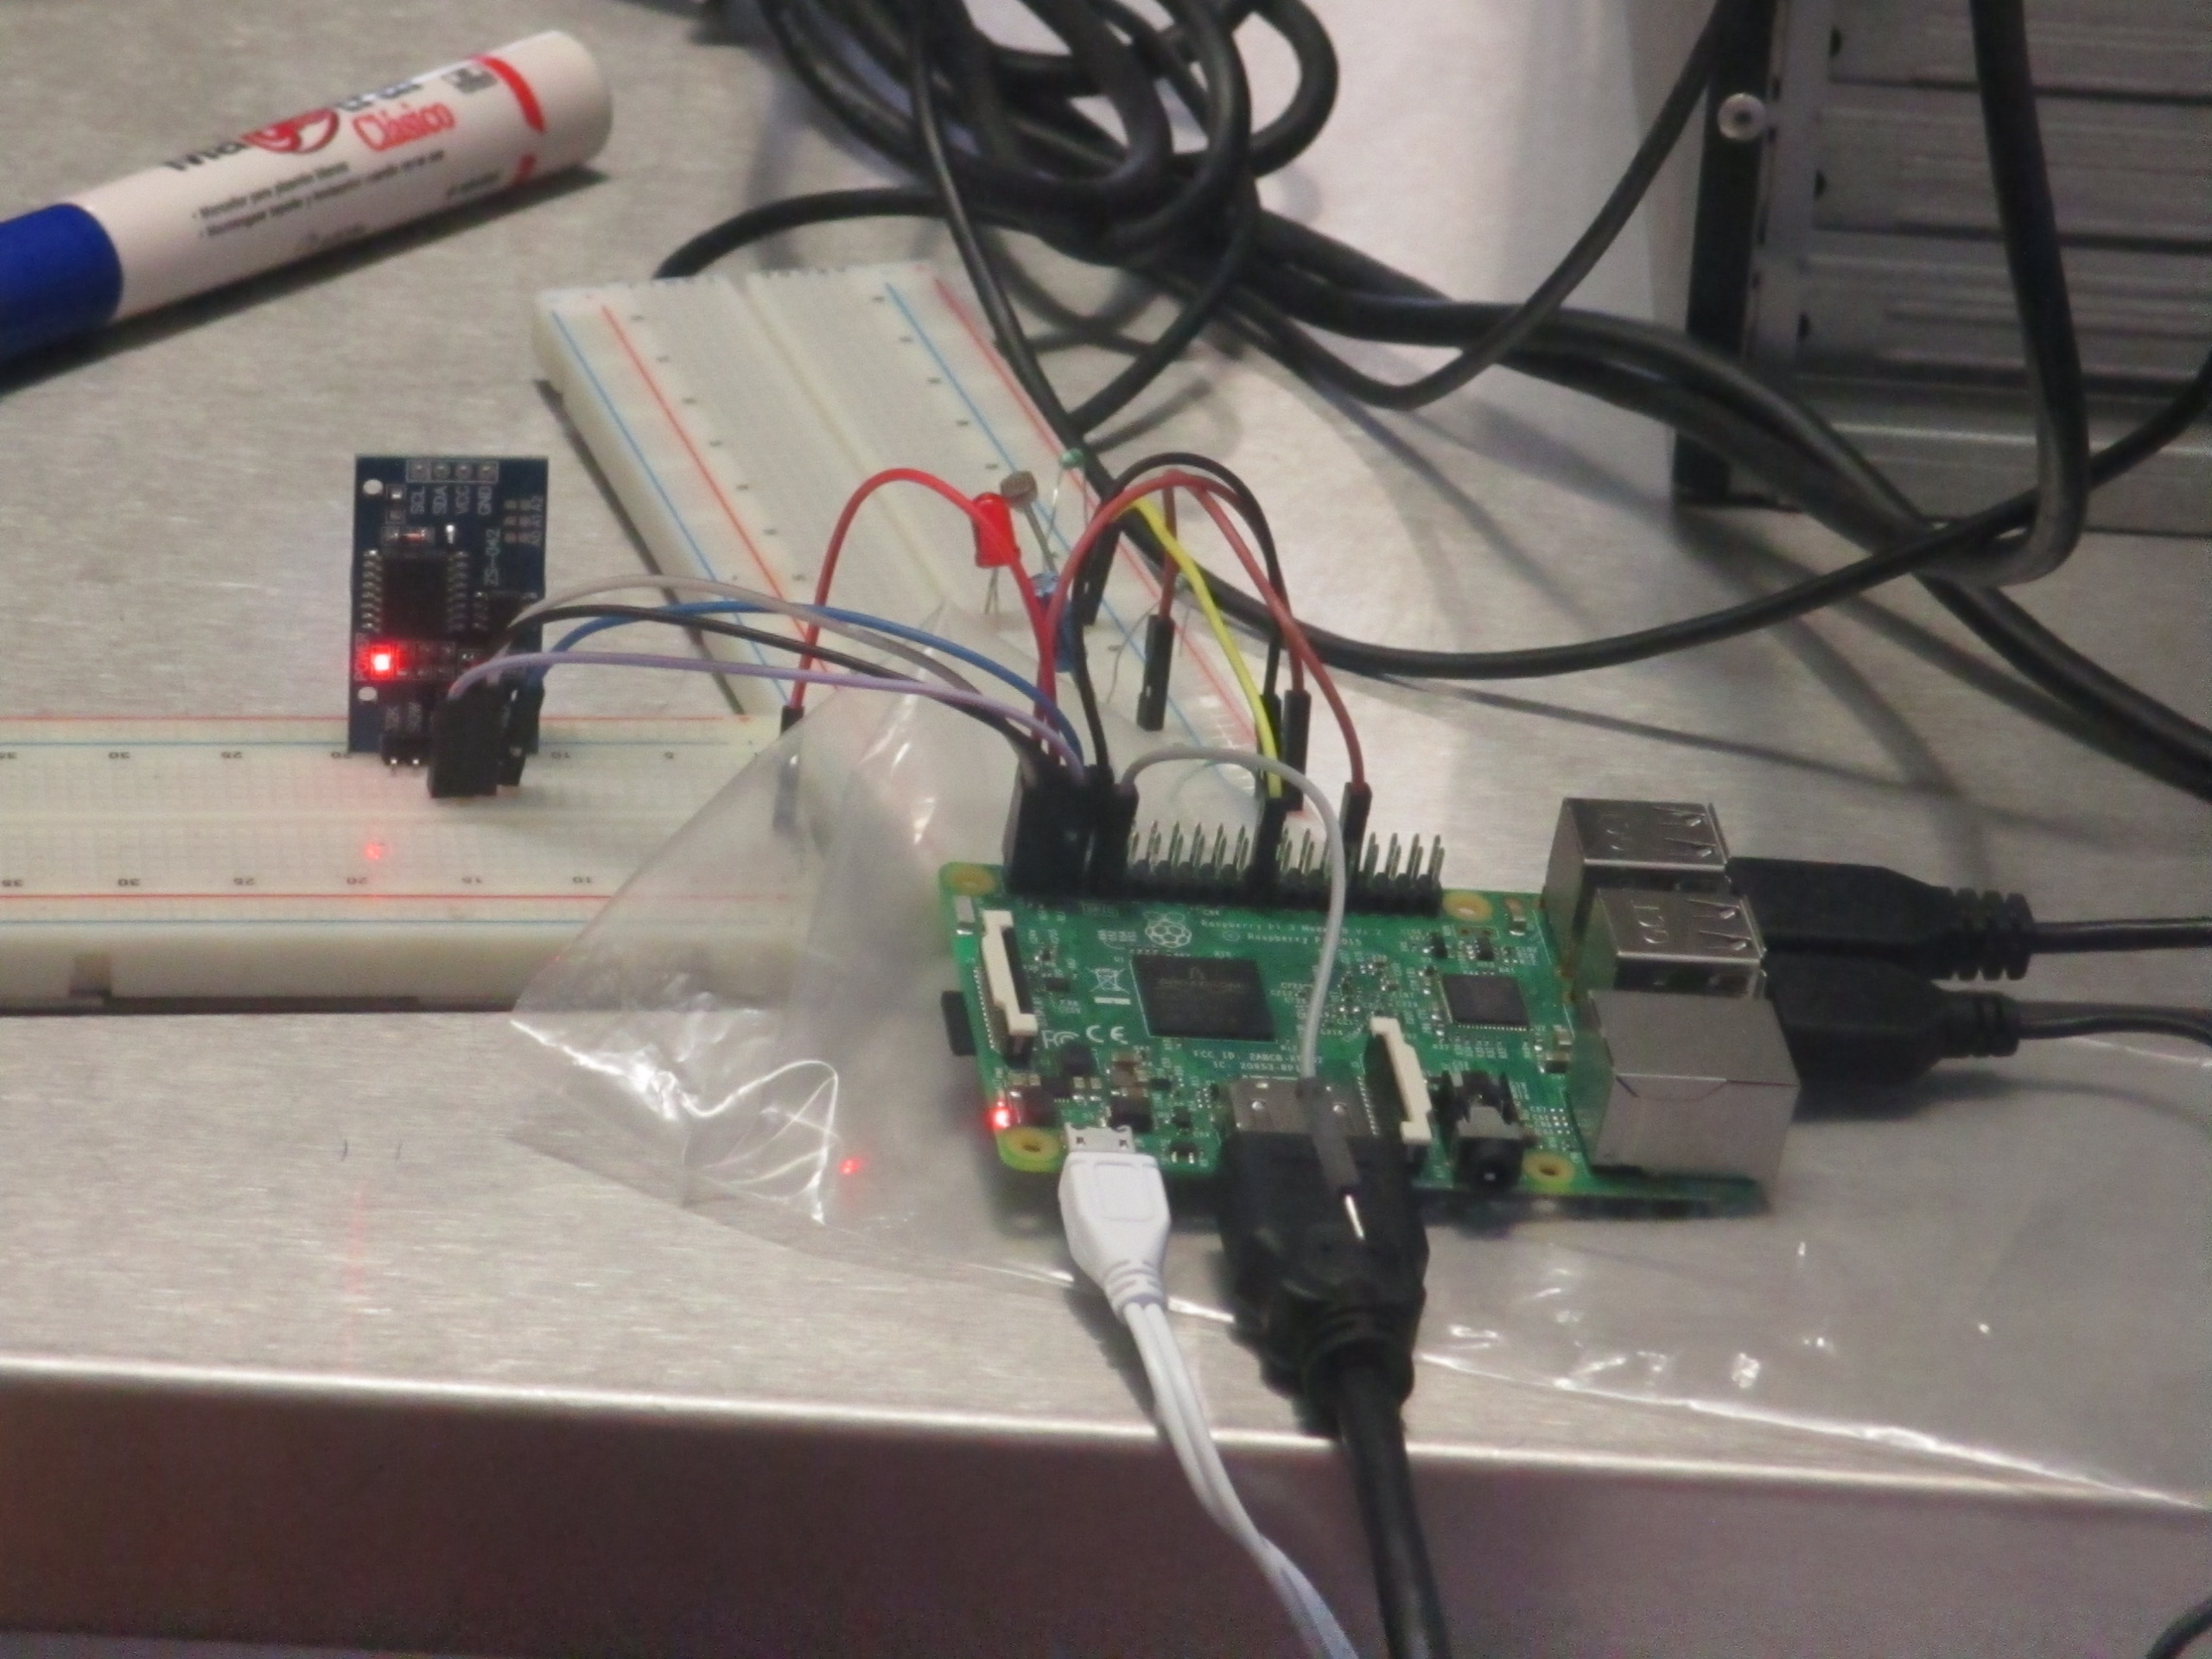
\includegraphics[width=8cm]{r2}
	\end{center}
	\caption{Prueba 1}
	\label{r2}
\end{figure} 

En la figura \ref{r3} se observa la implementaci\'on de la fotoresistencia con la raspberry. 
\begin{figure}[H]
	\begin{center}
		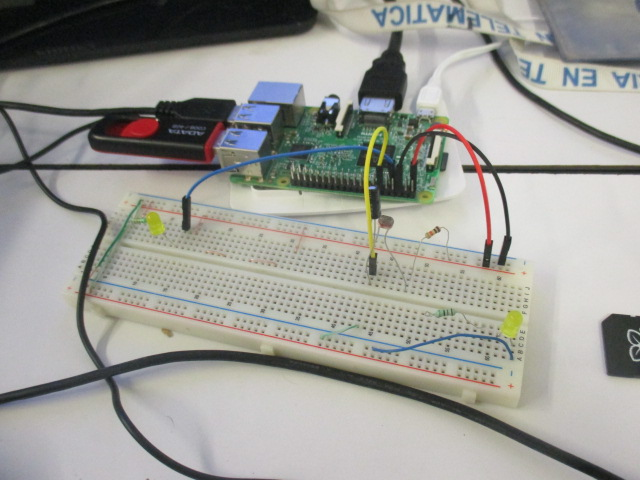
\includegraphics[width=8cm]{r3}
	\end{center}
	\caption{Prueba}
	\label{r3}
\end{figure} 


\subsubsection{Control de los sensores del sistema de riego con Raspberry}
Para poner en funcionamiento los sensores en la raspberry, se c\'odificaron una serie de pasos de cada uno de estos sensores, cabe mencionar que cada uno se realiz\'o por separado para analizar su comportamiento y verificar errores. En la figura \ref{r1} se puede observar la codificaci\'on en el sistema operativo de la raspberry.
\begin{figure}[H]
\begin{center}
	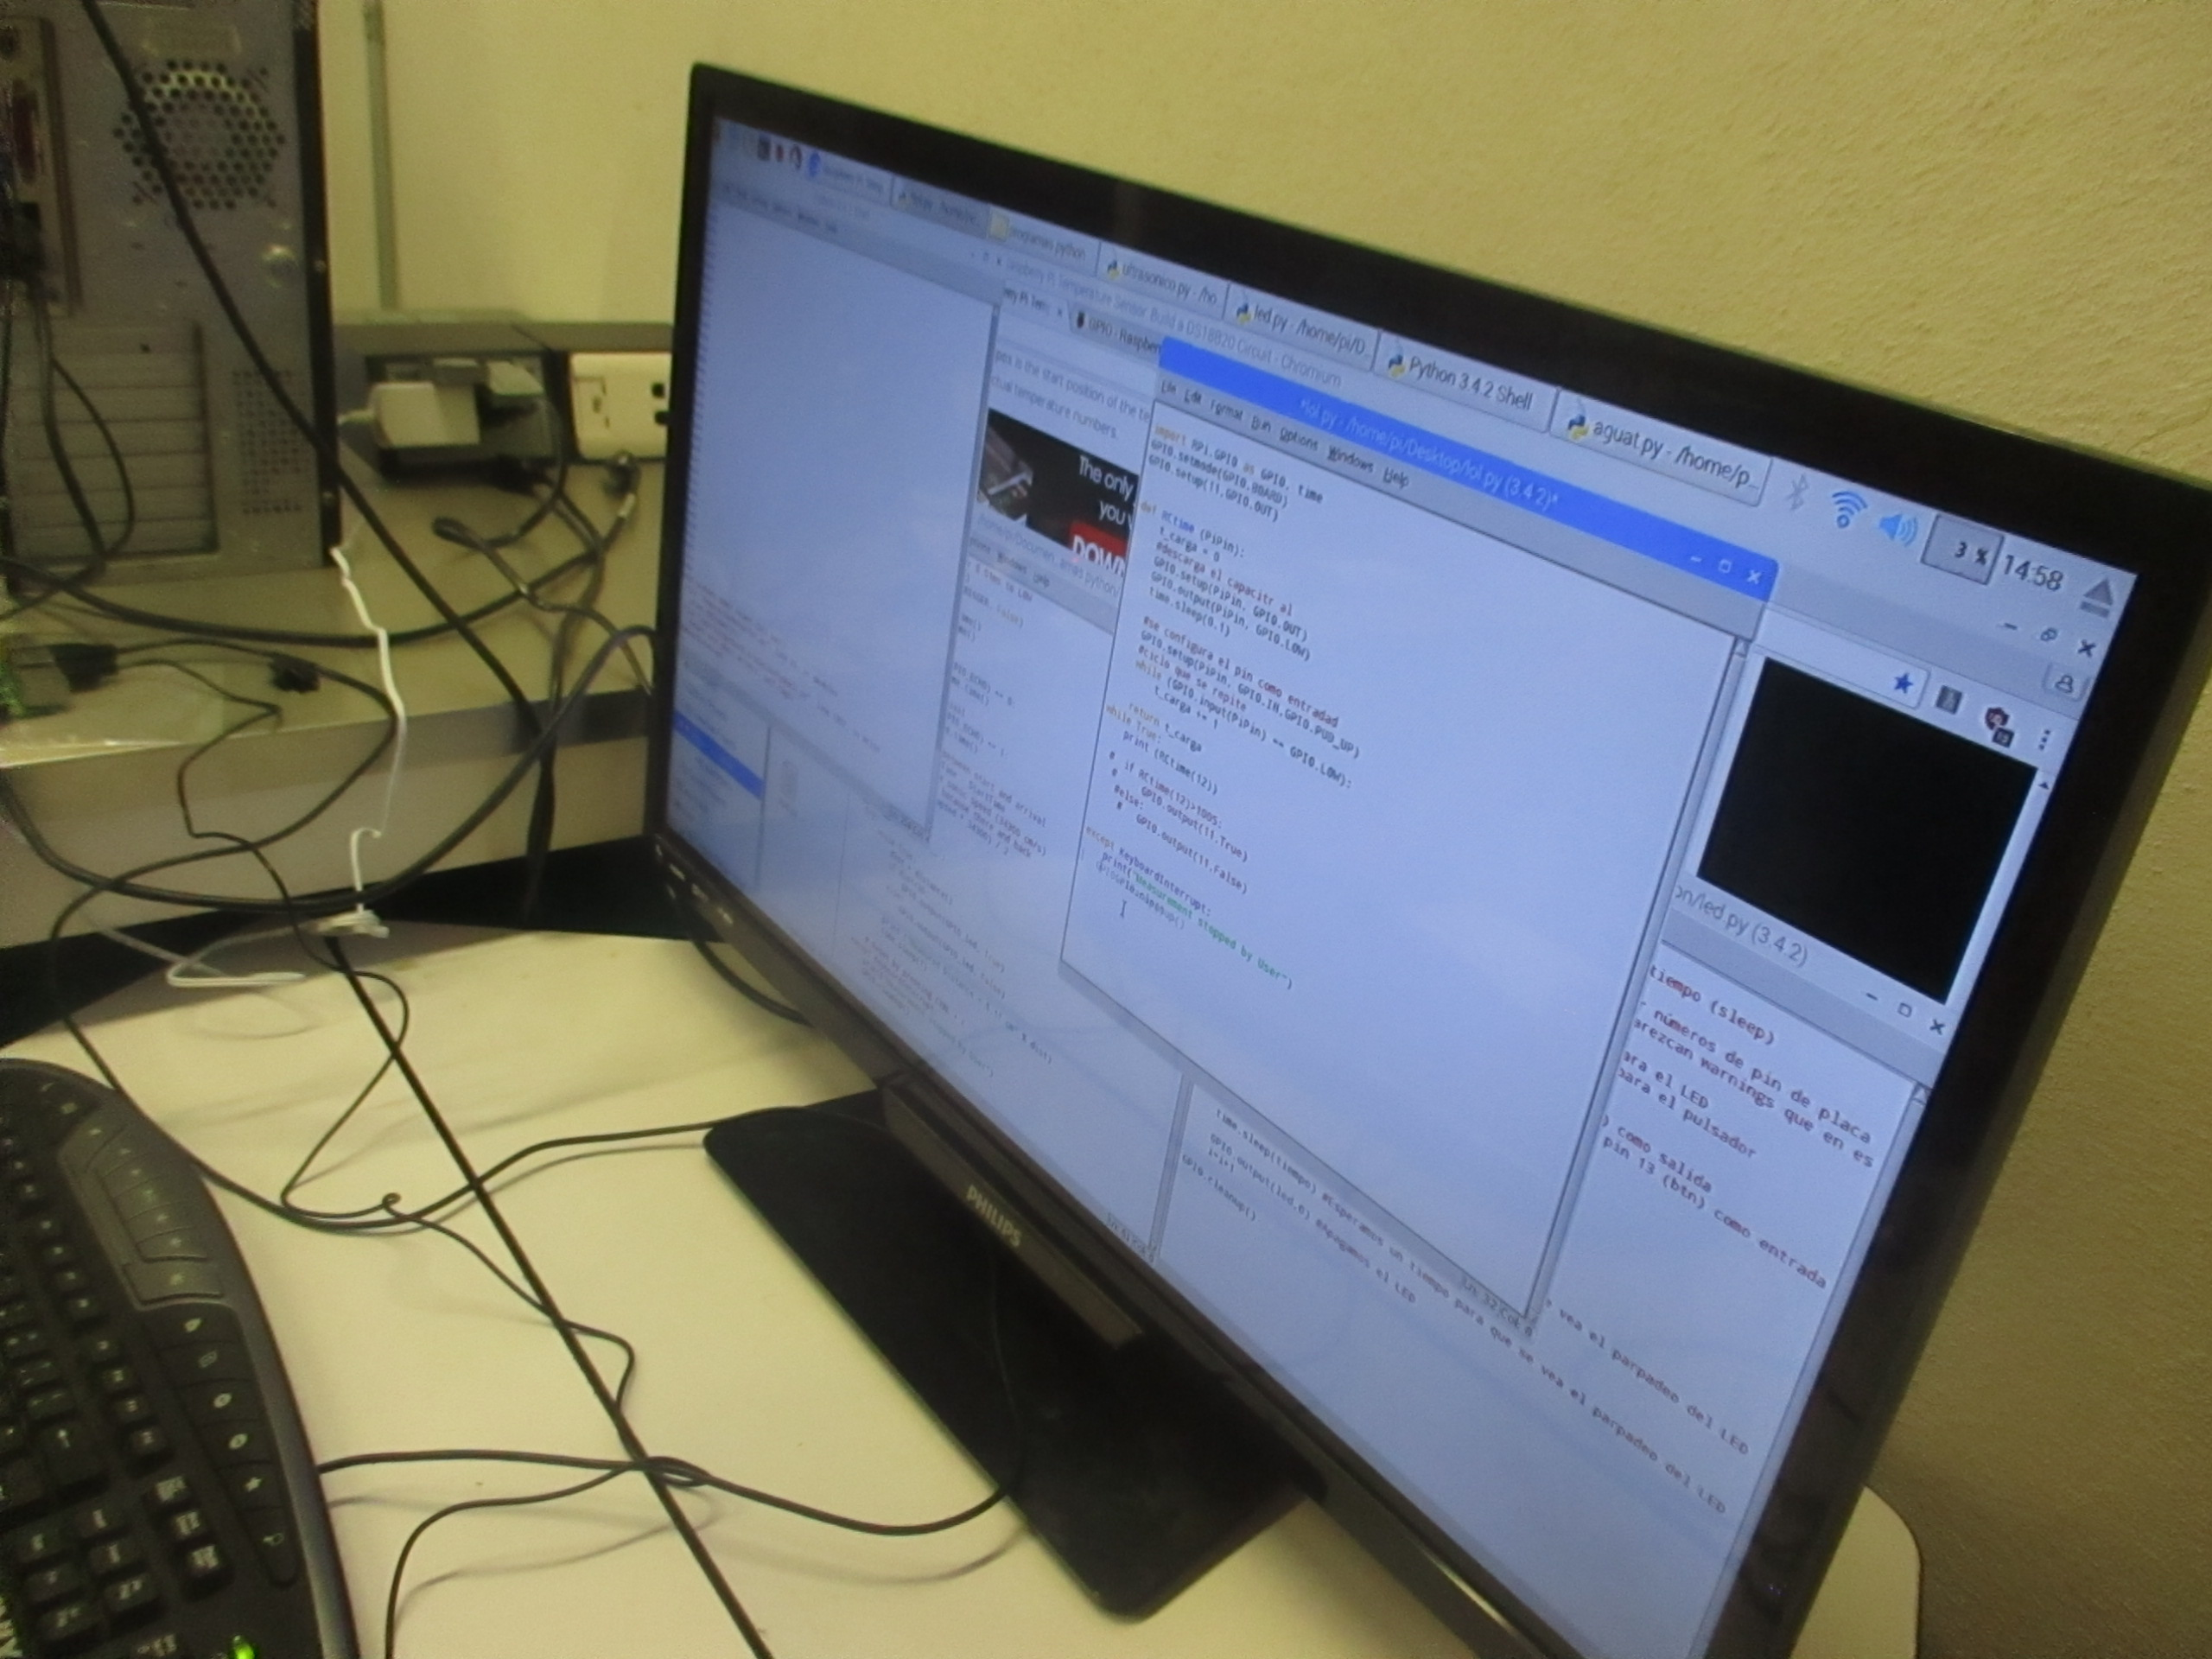
\includegraphics[width=9cm]{r1}
\end{center}
	\caption{Prueba 1}
	\label{r1}
\end{figure} 

En la figura \ref{r4} se muestran uno de los resultados obtenidos al probar el sensor de flujo de agua, mostrando los litros que pasan a trav\'es de este. 
\begin{figure}[H]
	\begin{center}
		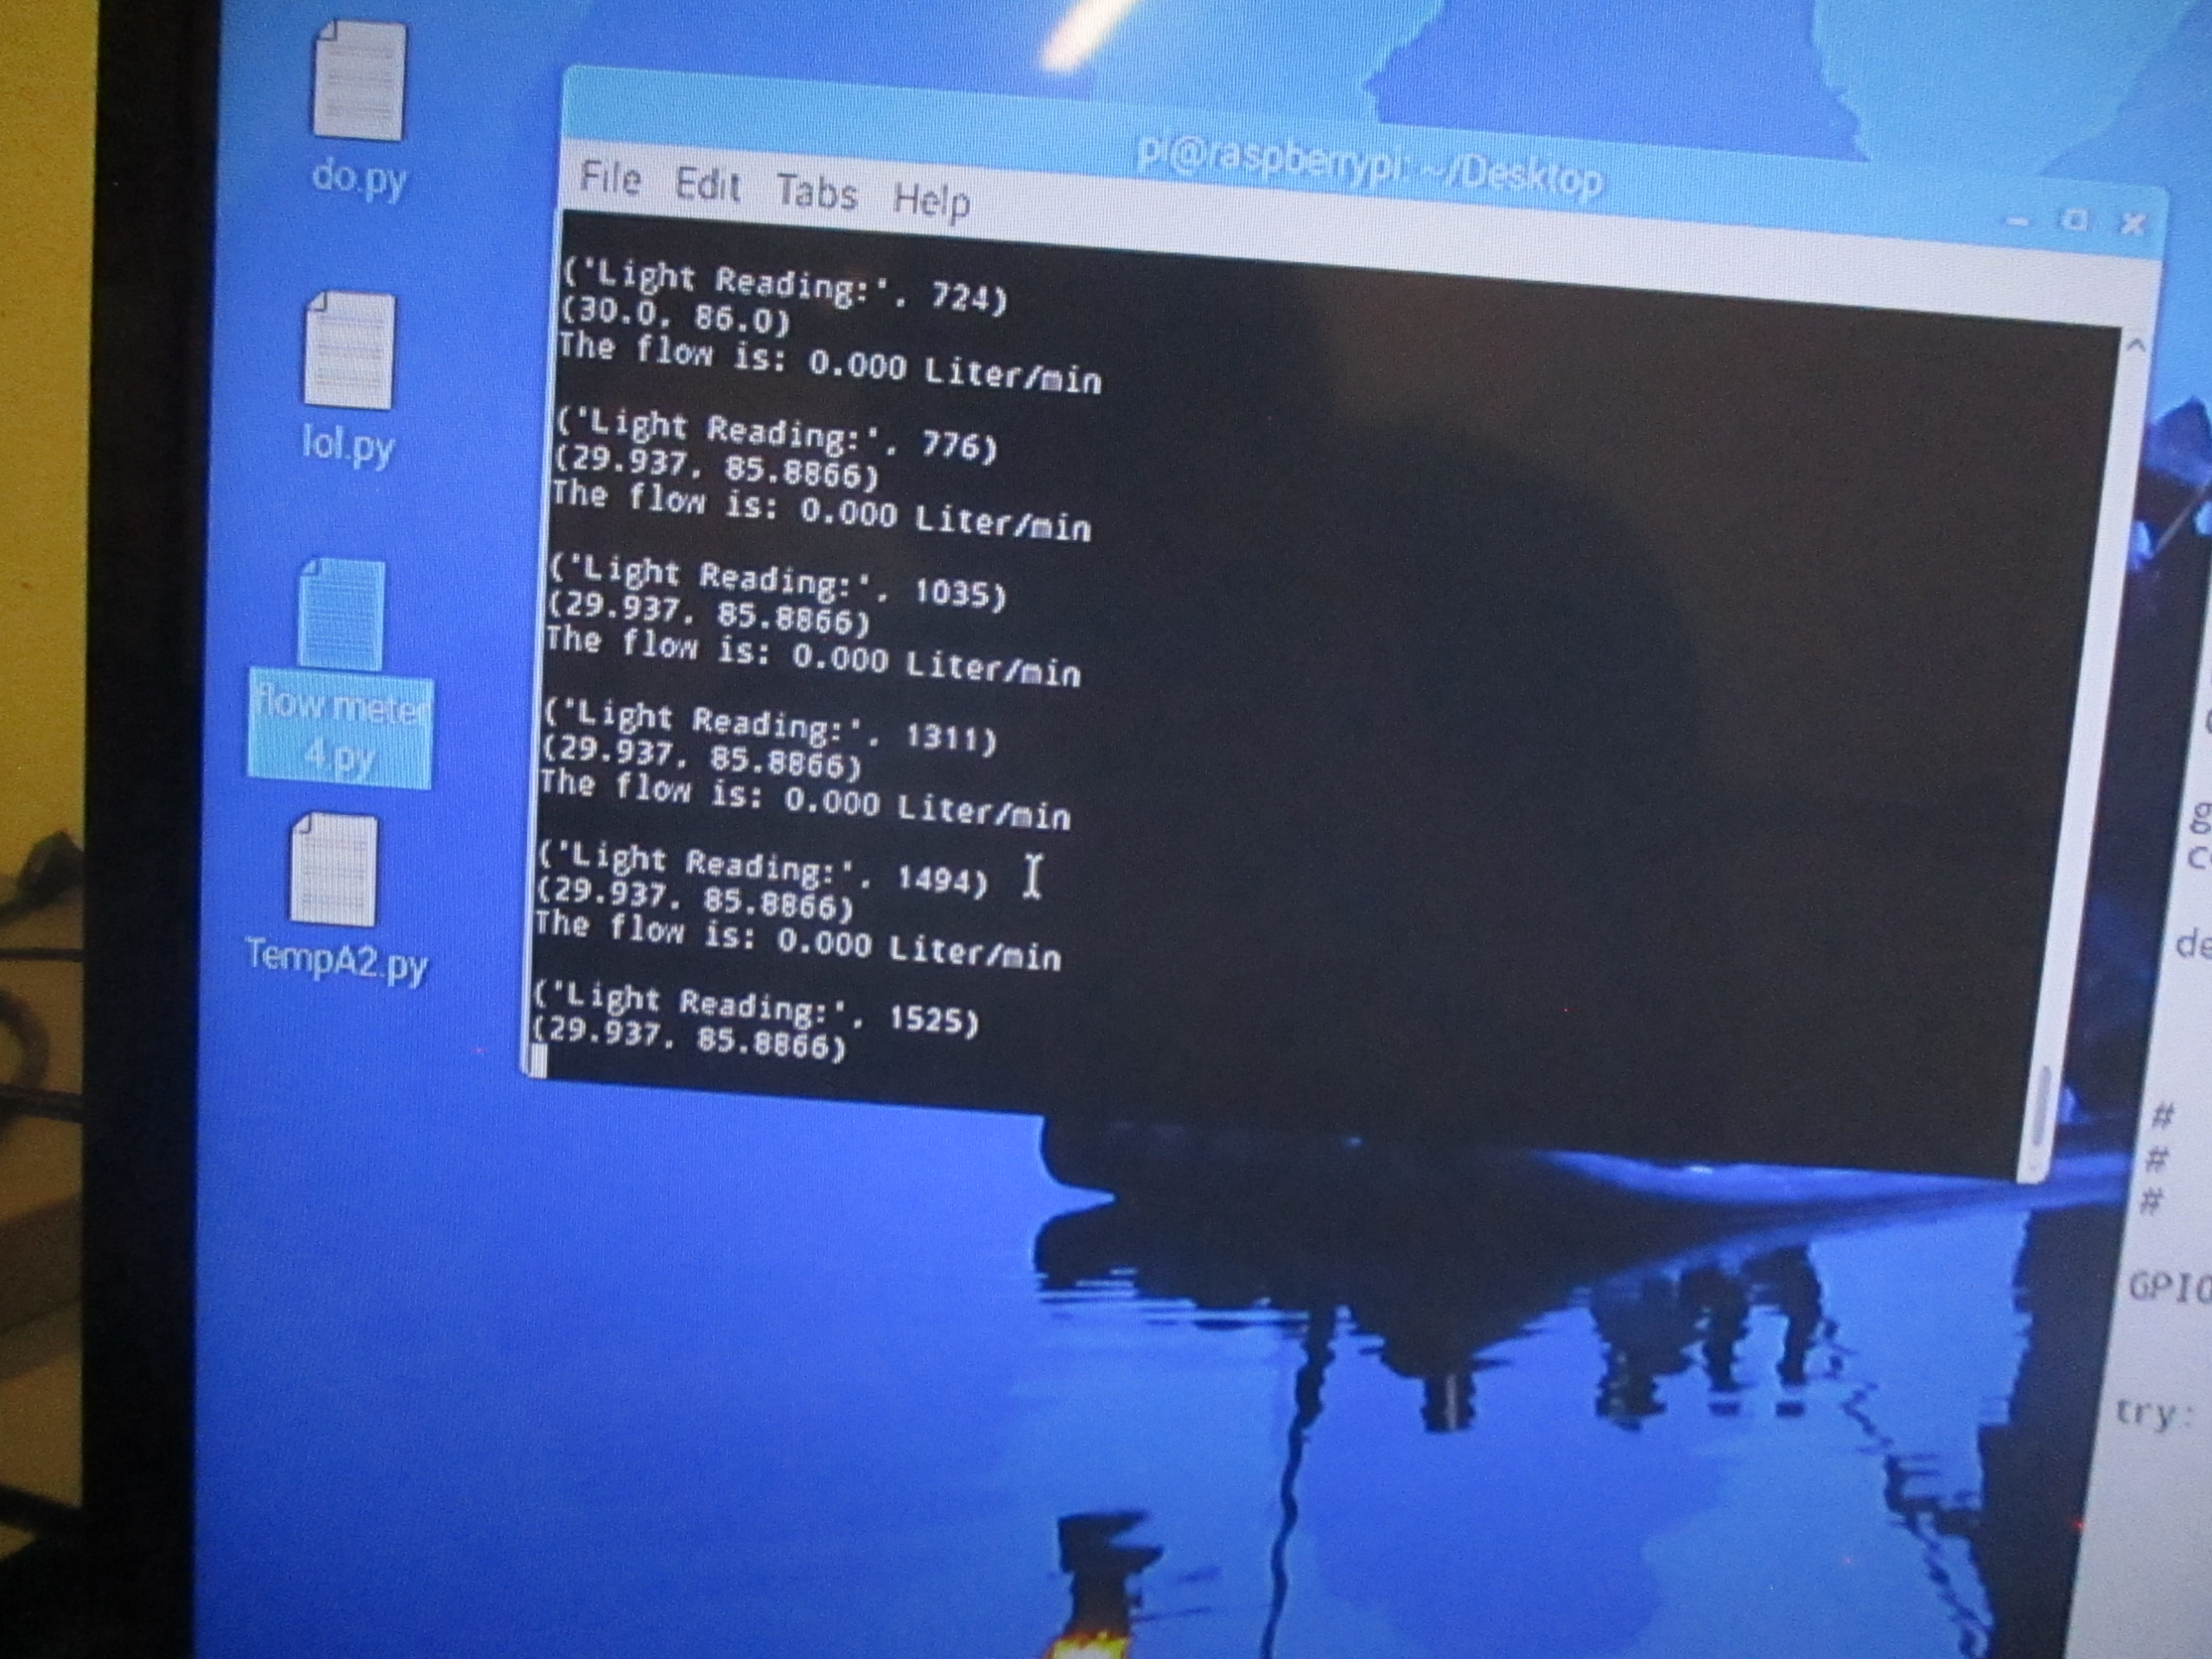
\includegraphics[width=9cm]{r4}
	\end{center}
	\caption{Prueba 2}
	\label{r4}
\end{figure} 

En la siguiente figura se presenta un muestre del funcionamiento de uno de los sensores del cual se hizo un an\'alisis para comprobar su efectivo funcionamiento.
\begin{figure}[H]
	\begin{center}
		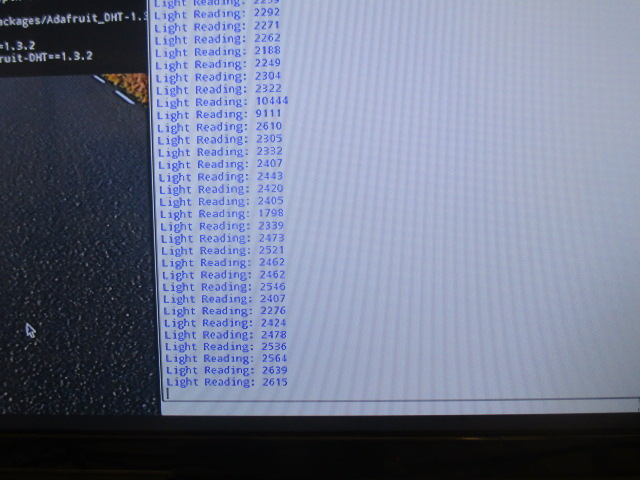
\includegraphics[width=9cm]{r12}
	\end{center}
	\caption{Prueba 3}
	\label{r12}
\end{figure} 


